\documentclass[conference]{IEEEtran}
\usepackage{cite}
\usepackage{amsmath,amssymb,amsfonts}
\usepackage{algorithm}
\usepackage{algorithmic}
\usepackage{graphicx}
\usepackage{textcomp}
\usepackage{xcolor}
\usepackage{booktabs}
\usepackage{hyperref}

\begin{document}

\title{Proactive Comfort Agent: Full Self-Driving Home Orchestration\\
\large Technical Specification Document (Phase 2 -- Deliverable B)}

\author{
\IEEEauthorblockN{Ha Yun Kim}
\IEEEauthorblockA{\textit{Dept. of Information Systems} \\
\textit{Hanyang University}\\
Seoul, Korea \\
hykim1215@hanyang.ac.kr}
\and
\IEEEauthorblockN{Soo Young Song}
\IEEEauthorblockA{\textit{Dept. of Information Systems} \\
\textit{Hanyang University}\\
Seoul, Korea \\
sys1109@hanyang.ac.kr}
\and
\IEEEauthorblockN{Ruitan Sun}
\IEEEauthorblockA{\textit{Dept. of Information Systems} \\
\textit{Hanyang University}\\
Seoul, Korea \\
sunruitan2024@126.com}
\and
\IEEEauthorblockN{Tang Bin}
\IEEEauthorblockA{\textit{Dept. of Information Systems} \\
\textit{Hanyang University}\\
Seoul, Korea \\
tbrobo99@outlook.com}
}

\maketitle

\begin{abstract}
Modern smart homes present usability and sustainability barriers when users must manage disconnected appliance apps, monitor indoor environmental hazards, and coordinate high-wattage operations. We propose \textbf{FSD-Home (Full Self-Driving Home Orchestration)}, a proactive orchestration system designed for inclusive, zero-labor, and energy-conscious living. By evaluating real-time IoT telemetry streams (ambient temperature, humidity decay, appliance power draw, and compressor duty cycles) alongside household schedules, FSD-Home predicts indoor environmental and energy risks---such as post-wash mold buildup, kitchen thermal spikes, and peak electricity surges---before they escalate. To ensure safety, sustainability, and user autonomy, the system introduces a Tesla-inspired Risk-Graded Framework: Level 1 eco-efficiency and environmental adjustments run automatically with plain-language updates, while Level 2 high-load or schedule-altering operations require explicit, per-action user approval via a touch-first, accessible interface overlay backed by an append-only audit trail.
\end{abstract}

\begin{IEEEkeywords}
Smart Home Orchestration, FSD-Home, Full Self-Driving Home, Risk-Graded Autonomy, Energy Load-Balancing, Environmental Sustainability, Level 1 and Level 2 Control, Functional Safety, LG ThinQ Ecosystem.
\end{IEEEkeywords}

\section{Introduction}

\subsection{Motivation}
Smart home appliances are ubiquitous today, but having more features does not automatically ensure a seamless or energy-efficient experience for every member of a household \cite{msit2026}. Complex menus, fragmented mobile applications, and lack of cross-device coordination create unnecessary cognitive burden \cite{moneytoday2026}, with over 67\% of surveyed consumers reporting friction with hidden menus and unclear controls \cite{maeil2026}. At the same time, routine household oversights cause significant safety, indoor air quality, and energy-waste issues: 35.3\% of residential fires start from unattended cooking \cite{seoulfire2020, nfa2025}; wet laundry left in closed washers quickly leads to mold and bacterial growth requiring energy-intensive sanitizing wash cycles \cite{epa2022, who2009}; and uncoordinated high-wattage appliance use drives peak-hour electricity surges and wasted HVAC cooling.

\subsection{Problem Statement}
Current smart home apps like LG ThinQ work in reactive silos \cite{lgspec2026}. They wait for manual button taps or send passive alerts (such as ``Cycle Finished''), leaving household members to diagnose environmental or energy issues themselves \cite{pradhan2020}. More importantly, appliances do not share thermodynamic or power-load awareness across rooms. When someone bakes in a hot oven while running a dryer, kitchen temperatures surge, forcing the refrigerator compressor and air conditioner to run at maximum duty cycles and draw peak electricity without coordinated pre-cooling, ventilation, or load interruption \cite{ashrae2023}. FSD-Home solves this by combining continuous sensor tracking with automated cross-appliance environmental and energy orchestration.

\subsection{Related Software}
Current commercial tools offer strong single-device features: LG AI DD\textsuperscript{TM} senses fabric softness via motor torque; LG ezDispense\textsuperscript{TM} automates detergent dosing; and LG ThinQ ON / ThinQ Claw provides conversational voice hubs \cite{lgwhitepaper2024, lgspec2026}. Samsung's Bespoke AI sends lifestyle pattern notifications \cite{samsung2026a, samsung2026b}. However, none of them coordinate thermal load, moisture prevention, and electricity demand across multiple devices \cite{yuan2024}. FSD-Home introduces three main contributions: (1) explicit predictive risk scores for indoor mold hygiene (MRI) and kitchen thermal/power overload (TOI), (2) a Tesla-inspired Level 1 / Level 2 autonomy model with per-action confirmation, energy-saving pre-cooling/load interruption, and safe standby fallback, and (3) an inclusive, touch-first overlay designed around WCAG 2.2 contrast and touch targets \cite{wcag2023}.

\section{Requirements Overview}

\subsection{Functional Requirements (FR)}
\begin{itemize}
    \item \textbf{FR-1 (Real-Time Environmental \& Power Telemetry Perception):} Continuously sample indoor temperature, humidity, drum moisture decay, door contact, household presence (\texttt{user\_home}), compressor duty cycle, and wattage at 1~Hz.
    \item \textbf{FR-2 (Predictive Environmental Hazard \& Energy Modeling):} Deterministically compute the Mold Risk Index (MRI) and Thermal Overload Index (TOI) to trigger interventions at a threshold of $50.0$.
    \item \textbf{FR-3 (Level 1 \& Level 2 Action Framework):} Enforce a strict 7-action whitelist separating automatic eco/comfort adjustments (Level 1) from per-action approval-gated interventions (Level 2).
    \item \textbf{FR-4 (Inclusive UI/UX \& Per-Action Consent Overlay):} Provide WCAG 2.2 compliant touch controls, separate approval prompts per Level 2 action, supplementary TTS voice prompts, manual quiet-period status review, and truthful adapter-grounded result messages.
    \item \textbf{FR-5 (Fail-Safe Default \& Pre-Execution Safety Policy):} Enforce a 300-second approval expiration defaulting to safe standby, pre-execution state/risk revalidation, cooktop presence and auto-off safeguards, and dryer restart reminders.
    \item \textbf{FR-6 (Structured Append-Only Audit Trail):} Maintain an immutable SQLite \texttt{audit\_log} linking risk triggers, per-action approvals (\texttt{approval\_id}), and actual device execution outcomes.
\end{itemize}

\subsection{Non-Functional Requirements (NFR)}
\begin{itemize}
    \item \textbf{NFR-1 (Latency \& Architectural Decoupling):} Complete deterministic local risk evaluation within $1.2\text{ ms}$ per 1~Hz tick ($30\text{ ms}$ tick budget) while isolating cloud LLM reasoning ($2.0\text{--}3.0\text{ s}$) behind a 180-second cooldown and rule-based fallback.
    \item \textbf{NFR-2 (Simulation Containment \& Verification):} Validate system behavior locally without physical appliance hardware using deterministic JSON/CSV telemetry streams, automated unit tests, and latency benchmarks.
\end{itemize}

\section{Development Environment}

\subsection{Choice of Software Development Platform}
The FSD-Home backend system is developed using \textbf{Python 3.10+} (targeting standard CPython 3.11 execution) without heavy external framework dependencies for core processing.
\begin{itemize}
    \item \textbf{Backend Runtime:} Built with Python standard library modules (\texttt{http.server}, \texttt{threading}, \texttt{sqlite3}) to maintain lightweight execution, high portability, and fast cold-start performance.
    \item \textbf{Frontend UI:} Developed using vanilla HTML5, CSS3, and ES6 JavaScript (no-build step, zero external dependencies). It interacts with the backend via HTTP REST endpoints (\texttt{GET /api/proactive}, \texttt{GET /api/approvals}, \texttt{POST /api/approvals/<id>/confirm}).
    \item \textbf{Storage and Persistence:} SQLite 3.43 utilizing Write-Ahead Logging (WAL) mode for transactional isolation, audit decision logs, and user preference state tracking.
    \item \textbf{Target Operating Environment:} Tested locally on Windows 11 (AMD Ryzen 7 5800H, 16\,GB RAM) without requiring discrete GPU acceleration. Designed for cross-platform portability across Linux (Ubuntu 22.04 LTS) and ARM-based single-board devices (e.g., Raspberry Pi 4, OpenWrt routers).
    \item \textbf{Cloud Hybrid Architecture:} While real-time risk checks run deterministically on local infrastructure in $1.2\text{ ms}$, LLM reasoning calls out asynchronously to OpenAI-compatible cloud endpoints (Zhipu GLM-4-Flash / vLLM API).
    \item \textbf{Version Control:} Managed via Git and hosted on GitHub (\url{https://github.com/tbrobo99/proactive-senior-care-comfort-agent}).
\end{itemize}

\subsection{Software and Algorithms in Use}
The system decouples real-time physical risk perception from LLM decision reasoning:
\begin{itemize}
    \item \textbf{Deterministic Risk Engines (\texttt{app/risk.py}):} Evaluates Mold Risk Index (MRI) and Thermal Overload Index (TOI) using closed-form thermodynamic models and 30-minute least-squares linear trend forecasting.
    \item \textbf{OpenAI-Compatible LLM Inference:} Integrates with Zhipu AI \texttt{glm-4-flash} (or local vLLM endpoints) for intent resolution and action candidate selection.
    \item \textbf{Deterministic Safety Gating (\texttt{app/policy.py}):} Restricts LLM output via a strict 7-action candidate whitelist divided into Level 1 (Autonomous) and Level 2 (Approval Required) tiers. Unknown or malformed action names are rejected and logged rather than executed.
\end{itemize}

\subsection{Cost Estimation}
\begin{table}[htbp]
\caption{Cost Estimation}
\begin{center}
\begin{tabular}{llr}
\toprule
\textbf{Item} & \textbf{Specification} & \textbf{Cost} \\
\midrule
Development HW & Existing Ryzen 7 PC & \textwon 0 \\
Core Software & Python 3.11, SQLite (Open-source) & \textwon 0 \\
Cloud API / LLM & Zhipu GLM-4-Flash / vLLM API & \textwon 0 (Free version) \\
Deployment & Local / Edge Simulation & \textwon 0 \\
\midrule
\textbf{Total Estimated Cost} & & \textbf{\textwon 0} \\
\bottomrule
\end{tabular}
\end{center}
\end{table}

\subsection{Task Distribution}
\begin{table}[htbp]
\caption{Role Assignments}
\begin{center}
\begin{tabular}{llp{4.3cm}}
\toprule
\textbf{Role} & \textbf{Assigned Member} & \textbf{Task Description \& Responsibilities} \\
\midrule
User & Ruitan Sun & Identify user needs, provide feedback, and help ensure the service meets user expectations. \\
Customer & Soo Young Song & Functional safety boundaries, Level 2 approval threshold definitions, audit log schema. \\
Software Developer & Tang Bin & General backend part: Agentic loop (\texttt{proactive.py}), risk engine (\texttt{risk.py}), telemetry generator (\texttt{sensors.py}). \\
Development Manager & Ha Yun Kim & System architecture design, LaTeX document formatting, UI design and accessibility validation. \\
\bottomrule
\end{tabular}
\end{center}
\end{table}

\section{Specifications}

\subsection{System Architecture Overview}
Fig.~\ref{fig:arch} illustrates the decoupled FSD-Home pipeline, separating 1~Hz deterministic telemetry evaluation and safety whitelisting from asynchronous cloud LLM ranking, per-action Level 2 approval modals, and append-only audit logging.

\begin{figure}[htbp]
\centering
\fbox{\parbox{0.94\columnwidth}{\footnotesize\ttfamily
[1 Hz Telemetry Stream: app/sensors.py]\\
Temp | Humidity | Door | Power (W) | Fridge Duty | user\_home\\
\hspace*{3em}$\downarrow$ (1.2 ms deterministic check)\\
{[Deterministic Risk \& Energy Engine: app/risk.py]}\\
MRI >= 50.0 (Mold Risk) \quad | \quad TOI >= 50.0 (Thermal/Load)\\
\hspace*{3em}$\downarrow$\\
{[Safety Whitelist \& Policy Gate: app/policy.py]}\\
Reject Unknown Actions | Assign Level 1 vs. Level 2\\
\hspace*{1em}$\swarrow$ (Level 1: Eco/Comfort) \hspace*{2em} $\searrow$ (Level 2: High-Load/Heat)\\
{[LLM Ranker / Abstain]} \hspace*{3.5em} {[Per-Action Approval Queue]}\\
(2--3 s; 180 s cooldown) \hspace*{3.5em} (app/approval.py, 300s TTL)\\
\hspace*{1em}$\searrow$ \hspace*{10em} $\swarrow$ [Confirm] + Revalidate\\
{[Device Adapters \& Append-Only Audit Log: app/db.py]}\\
Write Intent $\rightarrow$ Execute Adapter $\rightarrow$ Log Outcome $\rightarrow$ Update UI
}}
\caption{FSD-Home decoupled sensing, safety gating, per-action Level 2 approval, and append-only audit architecture.}
\label{fig:arch}
\end{figure}

\subsection{FR-1: Real-Time Environmental \& Power Telemetry Perception}
The \texttt{SensorSimulator} class in \texttt{app/sensors.py} generates 1~Hz time-series IoT telemetry snapshots.
\begin{itemize}
    \item \textbf{Data Pipeline:} Every snapshot is appended to \texttt{data/sensors/readings.jsonl}, and the latest readings are rewritten to \texttt{data/sensors/latest.csv}.
    \item \textbf{Simulated Metrics:} Room temperatures ($^\circ$C), relative humidity (\%), drum moisture decay, appliance door contact, household presence (\texttt{user\_home}), refrigerator compressor duty cycle, and active power draw (W).
\end{itemize}

\subsection{FR-2: Predictive Risk \& Energy Modeling}
The risk assessment module (\texttt{app/risk.py}) computes MRI and TOI deterministically within $1.2\text{ ms}$ per tick to protect indoor air quality and prevent wasteful peak-load energy spikes:
\begin{equation}
\text{MRI} = \text{clamp}\left[(H - 70.0) \times 3.2 + (S \times 6.0) + \max(0, T - 24.0) \times 1.5\right]
\end{equation}
\begin{equation}
\text{TOI} = \text{clamp}\left[\frac{W}{25.0} + \max(0, T_k - 27.0) \times 6.0 + \max(0, D - 0.6) \times 60.0 + 15\,C\right]
\end{equation}
\begin{itemize}
    \item \textbf{Environmental \& Hygiene Optimization (MRI):} Prevents mold proliferation in sealed appliances early using low-wattage ventilation or dehumidification, avoiding harsh chemical cleaners and energy-heavy hot-water tub-clean cycles \cite{epa2022, who2009}.
    \item \textbf{Thermodynamic \& Energy Load Balancing (TOI):} Tracks concurrent heat wattage ($W$), kitchen temperature ($T_k$), and refrigerator compressor duty cycle ($D > 0.6$, signaling excess thermal strain) alongside scheduled cooking events ($C = 1$ when a cooking session starts within 30 minutes, otherwise $0$) \cite{ashrae2023}.
    \item \textbf{Trigger \& Tier Separation:} When either index reaches or exceeds its configured threshold ($50.0$), an intervention event is dispatched. The risk threshold determines \emph{whether} an intervention is considered, whereas the predefined action tier determines \emph{whether} the action runs automatically or requires user approval.
\end{itemize}

\subsection{FR-3: Level 1 \& Level 2 Action Framework}
The local rule engine (\texttt{app/policy.py}) strictly enforces a 7-action whitelist (Table~\ref{tab:whitelist}). Unknown actions are blocked and recorded in \texttt{audit\_log}.
\begin{itemize}
    \item \textbf{Level 1 (Autonomous Eco \& Comfort Actions):} Low-power, reversible actions execute immediately when selected---including proactive kitchen pre-cooling (\texttt{precool\_kitchen} prior to scheduled cooking so the AC compressor runs smoothly at high efficiency rather than surging against peak oven heat) and targeted ventilation/dehumidification.
    \item \textbf{Level 2 (Per-Action Confirmation Required):} High-load or schedule-interrupting operations---such as stopping the dryer (\texttt{stop\_dryer}) during thermal/power overload so high-wattage heating elements do not overlap with kitchen cooking---generate individual pending confirmation states in \texttt{app/approval.py}. In the current proactive flow, Level 2 interventions are triggered by thermal/power overload risk (TOI), whereas mold risk (MRI) produces Level 1 actions.
\end{itemize}

\begin{table}[htbp]
\caption{Proposed Whitelist}
\label{tab:whitelist}
\begin{center}
\begin{tabular}{lll}
\toprule
\textbf{Tier} & \textbf{Action} & \textbf{Device} \\
\midrule
L1 & \texttt{ventilate\_washer} & Washer, drum vent \\
L1 & \texttt{dehumidifier\_on} & Balcony dehumidifier \\
L1 & \texttt{purifier\_on} & Living-room purifier \\
L1 & \texttt{ventilate\_kitchen} & Range hood, fan high \\
L1 & \texttt{precool\_kitchen} & Kitchen AC to $24^\circ\text{C}$ \\
L2 & \texttt{stop\_dryer} & Dryer off; restart by hand \\
L2 & \texttt{preheat\_cooktop} & Cooktop on early \\
\bottomrule
\end{tabular}
\end{center}
\end{table}

\subsection{FR-4: Inclusive UI/UX and Interface Specification}
\begin{itemize}
    \item \textbf{Per-Action Level 2 Approval Modal:} Rendered dynamically via REST polling (\texttt{GET /api/approvals}). Each Level 2 action is presented with its own separate plain-language question and unique \texttt{approval\_id} so approving one action cannot authorize another.
    \item \textbf{Visual \& Touch Targets:} Text contrast exceeds $4.5:1$, and primary touch targets are $\ge 48 \times 48\text{ px}$ with clearly labeled \texttt{[Confirm]} and \texttt{[Decline]} buttons.
    \item \textbf{Real-Time Visual Countdown:} Displays a visible 300-second countdown timer. Upon timeout, the request transitions to \texttt{expired} without altering appliance state.
    \item \textbf{Touch-First Multimodal Support:} Touch buttons serve as the primary consent method. Spoken prompts (via Web Speech API TTS) and visible text act as supplementary aids; silence, ambiguous speech, or prompt playback alone never count as consent.
    \item \textbf{Truthful Outcome Reporting \& Quiet-Period Status View:} Reports actual adapter outcomes (\texttt{completed}, \texttt{canceled}, or \texttt{failed}) with a concise reason, keeping technical telemetry in the audit log. During the 30-minute quiet period after a decline or timeout, users can still open the interface to manually check live risk status.
\end{itemize}

\subsection{FR-5: Fail-Safe Default Policy}
\begin{itemize}
    \item \textbf{300-Second Expiry \& Safe Standby:} Level 2 confirmation requests expire after 300 seconds (\texttt{APPROVAL\_TTL\_SECONDS}). Decline, expiry, late responses, or system restarts never execute pending Level 2 actions and initiate a 1,800-second (30-minute) quiet period for that risk kind.
    \item \textbf{Pre-Execution Revalidation \& Cooktop Safeguards:} Upon confirmation within 300 seconds, the engine re-verifies approval validity, active risk conditions, device state, and safety interlocks immediately before calling the device adapter. Because \texttt{preheat\_cooktop} prepares a scheduled meal rather than relieving the overload, it is revalidated against the meal instead of the risk score: execution requires verified household presence (\texttt{user\_home}), a cooking session still scheduled within 30 minutes, and the cooktop still off. After execution, an automatic shut-off interlock switches the cooktop off if cooking is not detected within 5 minutes of the scheduled start (\texttt{cooktop\_no\_cook\_timeout}, preventing wasted energy and fire hazards), and in any case after a 30-minute maximum continuous run time (\texttt{cooktop\_max\_runtime}).
    \item \textbf{Follow-Up Notification:} When \texttt{stop\_dryer} interrupts a cycle to relieve thermal and electrical overload, the system notifies the user once the risk clears so they can restart the dryer manually.
\end{itemize}

\subsection{FR-6: Structured Append-Only Audit Trail}
To ensure end-to-end traceability across risk evaluation, user consent, and hardware execution (\texttt{app/db.py}), the system maintains an append-only SQLite \texttt{audit\_log} table (protected against \texttt{UPDATE} and \texttt{DELETE} via database triggers):
\begin{itemize}
    \item \textbf{Linked Event Records:} Captures timezone-aware ISO 8601 timestamps, \texttt{event\_type} (e.g., \texttt{risk.triggered}, \texttt{approval.proposed}, \texttt{approval.confirmed}, \texttt{action.executed}, \texttt{action.failed}, \texttt{action.blocked}), \texttt{risk\_kind}, \texttt{risk\_score}, \texttt{action\_kind}, \texttt{tier}, \texttt{approval\_id}, \texttt{approval\_status}, \texttt{execution\_status}, \texttt{decision\_source}, and \texttt{channel}.
    \item \textbf{Write-Before-Act Integrity:} Action intent is recorded prior to invoking the device adapter, and actual adapter outcomes are logged immediately afterward. If audit persistence fails prior to a Level 2 execution, the action is aborted.
\end{itemize}

\subsection{Control Flow and Algorithmic Execution}
Algorithm~\ref{alg:control} defines the 1~Hz orchestration loop, per-action Level 2 approval queuing, and pre-execution revalidation.

\begin{algorithm}[htbp]
\caption{1~Hz Proactive Orchestration and Per-Action Approval}
\label{alg:control}
\begin{algorithmic}[1]
\STATE \textbf{function} \textsc{tick}() \COMMENT{1 Hz sampling; decisions may wait}
\STATE \quad $snap \leftarrow \text{sensors.snapshot}()$; $\text{sensors.record}(snap)$
\STATE \quad \textbf{for} $r \in [r \in \text{risk.evaluate}(snap, hist) \mid r.\text{score} \ge 50.0]$ \textbf{do}
\STATE \quad \quad \textbf{if} $\text{cooling}(r.\text{kind}) \lor \text{pending}(r.\text{kind})$ \textbf{then continue}
\STATE \quad \quad $\textsc{intervene}(r, snap)$ \COMMENT{may call the model}
\STATE \quad \textbf{for} $ap \in \text{approvals.expire\_due}()$ \textbf{do} \COMMENT{300s deadline check}
\STATE \quad \quad $\text{quiet}(ap.\text{risk\_kind}, 30\text{ min})$; $\text{report}(ap)$
\STATE
\STATE \textbf{function} \textsc{intervene}($r, snap$)
\STATE \quad $cands \leftarrow \text{policy.candidates}(r, snap)$ \COMMENT{whitelist}
\STATE \quad $chosen \leftarrow \text{decide}(r, cands)$ \COMMENT{LLM ranks L1 or abstains}
\STATE \quad \textbf{for} $c \in cands$ \textbf{do}
\STATE \quad \quad \textbf{if} $\text{tier\_of}(c) == \text{TIER2}$ \textbf{then}
\STATE \quad \quad \quad $\text{approval.propose}(c, \text{ttl}=300)$ \COMMENT{per-action ID}
\STATE \quad \quad \textbf{else if} $c \in chosen \land \text{revalidate}(c, snap)$ \textbf{then}
\STATE \quad \quad \quad $\text{run\_and\_log}(c)$
\STATE
\STATE \textbf{function} \textsc{on\_confirm}($approval\_id, channel$)
\STATE \quad $ap \leftarrow \text{approval.confirm}(approval\_id, channel)$
\STATE \quad \textbf{if} $ap \land \text{revalidate}(ap.\text{action}, \text{sensors.snapshot}())$ \textbf{then}

\STATE \quad \quad $result \leftarrow \text{audit.execute}(adapter, ap.\text{action})$ \COMMENT{intent, call, outcome}
\STATE \quad \quad $\text{report\_outcome}(ap, result)$
\end{algorithmic}
\end{algorithm}

\subsection{NFR-1 \& NFR-2: Latency Decoupling and Verification}
\begin{itemize}
    \item \textbf{Latency Budget (NFR-1):} Deterministic local sensor checks complete in $1.2\text{ ms}$ per 1~Hz tick (overall deterministic tick budget: $30\text{ ms}$). Cloud LLM reasoning runs within $2.0$--$3.0\text{ s}$ upon threshold breach, bounded by a 180-second cooldown ($\sim$40 calls/hour max). If model output is disabled, times out, or returns invalid JSON, deterministic rule defaults apply while keeping all Level 2 actions strictly approval-gated.
    \item \textbf{Simulation Containment \& Verification (NFR-2):} All telemetry, calendar schedules, and appliance adapters execute locally via synthetic JSON/CSV streams and are verified through automated unit test suites and latency/accuracy benchmark scripts (\texttt{tests/}, \texttt{eval/}).
\end{itemize}

% ======================================================================
\section{Architecture Design \& Implementation}

\subsection{Overall Architecture}
Fig.~\ref{fig:arch-impl} shows the implemented system as eleven software components. Each box names the component, its source location, its responsibility and its main classes or functions; each directed edge is labelled with the call that crosses it. Amber boxes and edges mark the safety path: every proposed action passes the whitelist in the Safety Policy, every Level~2 action passes the Approval Queue, and every device write --- from the proactive loop, from voice or text commands, from scheduled jobs and from the manual controls --- passes the Audit Gate before it reaches a Device Adapter.

The architecture keeps three properties that the requirements depend on. First, \emph{perception is deterministic}: the Sensor Simulator and the Risk Engine run on every 1~Hz tick without the language model in the path (NFR-1). Second, \emph{the model ranks but never authorizes}: the LLM Client only orders Level~1 candidates that the policy already produced, and any failure falls back to the rules (FR-3). Third, \emph{there is one door to the devices}: \texttt{audit.execute()} is the only function that calls \texttt{DeviceAdapter.apply()} on the action path, so intent and outcome are always recorded on either side of a device write (FR-6).

\begin{figure*}[t]
\centering
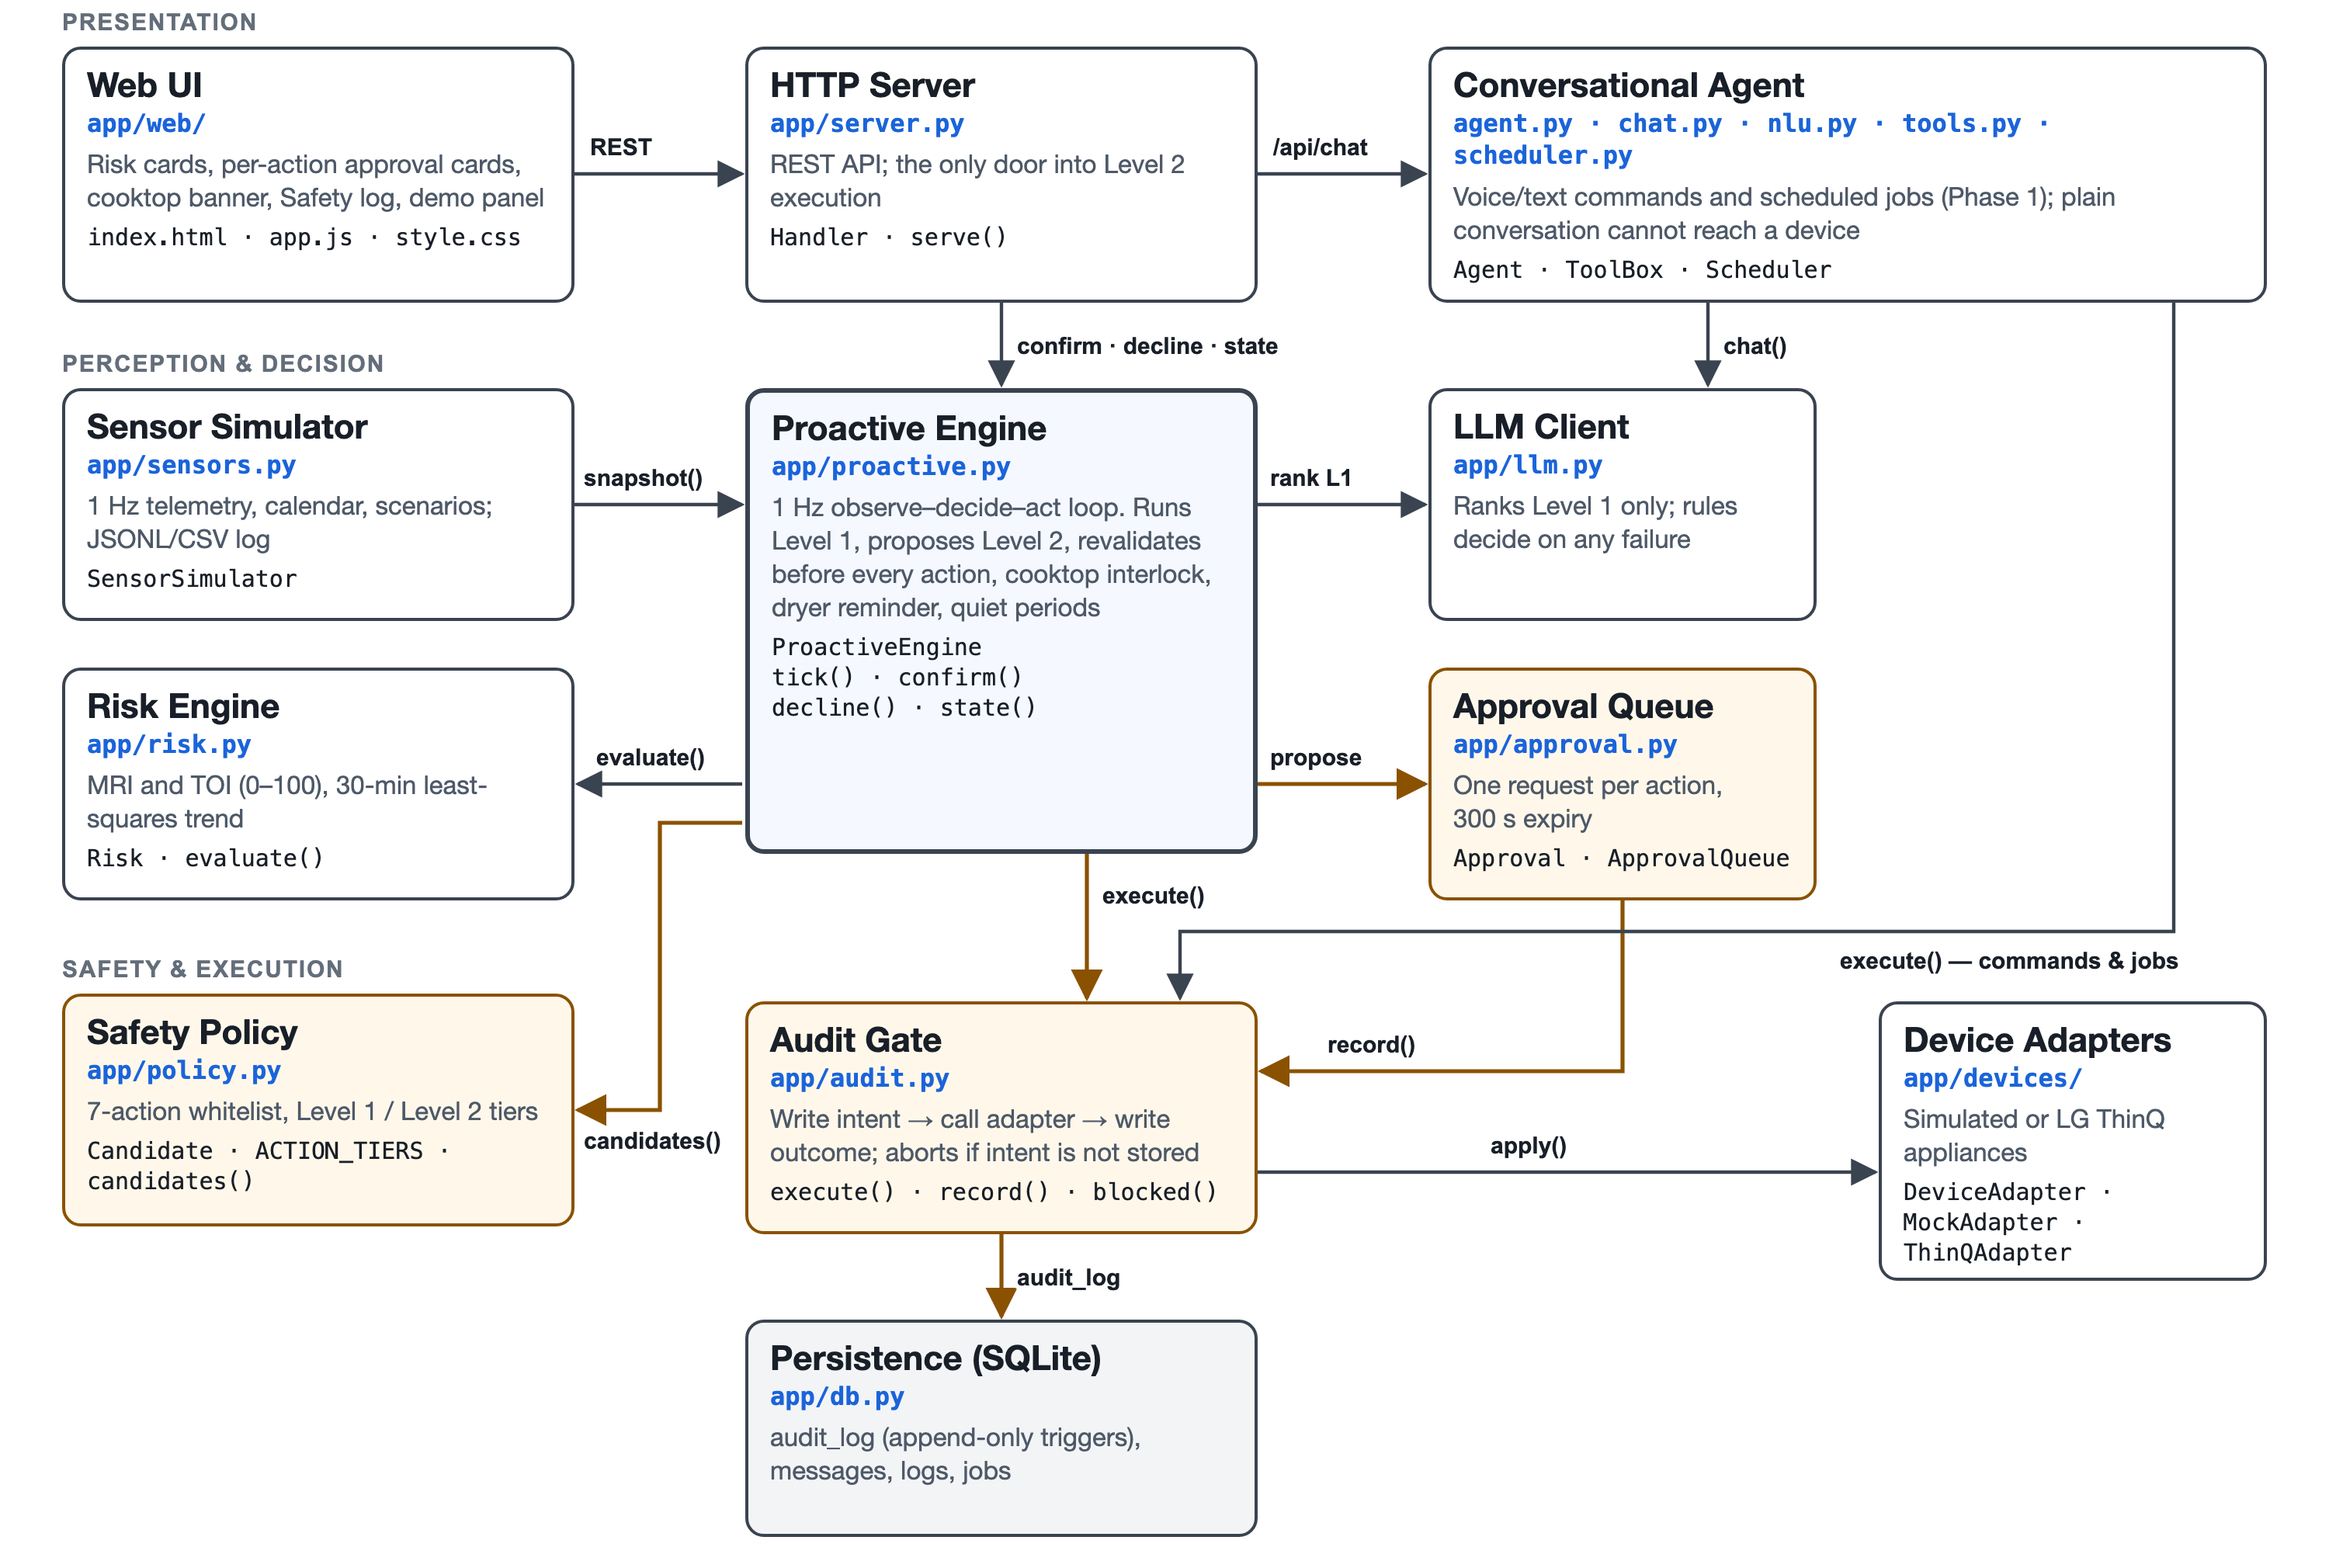
\includegraphics[width=0.92\textwidth]{figures/architecture.png}
\caption{Implemented FSD-Home architecture. Boxes are software components (title, location, responsibility, main classes); directed edges are labelled with the call that crosses them. Amber marks the safety path: whitelist, per-action approval, and the write-before-act audit gate.}
\label{fig:arch-impl}
\end{figure*}

\subsection{Directory Organization}
Table~\ref{tab:dirs} lists the source tree. The core runtime uses only the Python standard library; the optional LG ThinQ adapter needs the \texttt{thinqconnect} SDK, and the optional language model is reached over an OpenAI-compatible HTTP API.

\begin{table*}[t]
\caption{Directory Organization and Source Files}
\label{tab:dirs}
\centering
\footnotesize
\begin{tabular}{p{1.9cm}p{4.4cm}p{3.1cm}p{5.6cm}}
\toprule
\textbf{Directory} & \textbf{File names} & \textbf{Module (component)} & \textbf{Notes} \\
\midrule
\texttt{/} & \texttt{run.py}, \texttt{start.bat} & Entry point & Starts adapter, proactive engine, scheduler and web server; \texttt{--scenario}, \texttt{--port}, \texttt{--lan} \\
\texttt{app/} & \texttt{sensors.py} & Sensor Simulator & \texttt{SensorSimulator}: 1~Hz rooms, appliances, calendar, scenarios \\
\texttt{app/} & \texttt{risk.py} & Risk Engine & \texttt{Risk}, \texttt{mold\_risk()}, \texttt{thermal\_risk()}, \texttt{evaluate()} \\
\texttt{app/} & \texttt{policy.py} & Safety Policy & \texttt{Candidate}, \texttt{ACTION\_TIERS}, \texttt{candidates()}, \texttt{tier\_of()} \\
\texttt{app/} & \texttt{proactive.py} & Proactive Engine & \texttt{ProactiveEngine}: loop, revalidation, cooktop interlock, dryer reminder \\
\texttt{app/} & \texttt{approval.py} & Approval Queue & \texttt{Approval}, \texttt{ApprovalQueue}: per-action requests, 300~s expiry \\
\texttt{app/} & \texttt{audit.py}, \texttt{db.py} & Audit Gate, Persistence & \texttt{execute()}, \texttt{record()}, \texttt{blocked()}; SQLite schema with append-only triggers \\
\texttt{app/} & \texttt{llm.py} & LLM Client & OpenAI-compatible \texttt{chat()}; used for ranking and conversation \\
\texttt{app/} & \texttt{server.py} & HTTP Server & \texttt{Handler}: REST API and static files \\
\texttt{app/} & \texttt{agent.py}, \texttt{chat.py}, \texttt{nlu.py}, \texttt{tools.py}, \texttt{scheduler.py}, \texttt{agent\_loop.py}, \texttt{scenes.py}, \texttt{food.py} & Conversational Agent & Phase~1 voice/text commands, schedules and conversation; device writes go through the Audit Gate \\
\texttt{app/} & \texttt{config.py}, \texttt{build.py} & Configuration & Defaults, \texttt{config.json}, build stamp \\
\texttt{app/devices/} & \texttt{base.py}, \texttt{mock.py}, \texttt{thinq.py} & Device Adapters & \texttt{DeviceAdapter}, \texttt{MockAdapter} (11 simulated appliances), \texttt{ThinQAdapter} (dry-run by default) \\
\texttt{app/web/} & \texttt{index.html}, \texttt{app.js}, \texttt{style.css}, \texttt{sw.js} & Web UI & Dashboard, approval cards, Safety log, demo controls; no build step \\
\texttt{tests/} & \texttt{test\_phase2.py}, \texttt{test\_fr456.py}, \ldots & Unit tests & 276 tests; run on Windows and Linux in GitHub Actions \\
\texttt{eval/} & \texttt{run.py}, \texttt{latency.py}, \texttt{dataset.jsonl} & Benchmarks & Intent-parser regression and latency measurement \\
\texttt{docs/} & \texttt{*.tex}, \texttt{figures/} & Documentation & This paper, figures and screenshots \\
\bottomrule
\end{tabular}
\end{table*}

\subsection{Sensor Simulator (\texttt{app/sensors.py})}
\textbf{Purpose.} Provide the telemetry FR-1 asks for without physical appliances (NFR-2).
\textbf{Functionality.} \texttt{SensorSimulator} advances a small physical model once per second: an oven or cooktop heats the kitchen, the range hood and the air conditioner pull it back, the dryer warms the balcony, a sealed washer drum gains humidity while drum ventilation removes it, and the refrigerator's compressor duty cycle follows its external temperature probe. \texttt{note\_action()} feeds every executed command back into the model so that interventions have visible effects. \texttt{apply\_scenario()} loads the deterministic starting states used in the use cases (\texttt{idle}, \texttt{mold}, \texttt{oven}, \texttt{oven\_running}), and \texttt{record()} appends every snapshot to \texttt{data/sensors/readings.jsonl} and rewrites \texttt{latest.csv}. The day's cooking sessions are read from a local JSON calendar.
\textbf{Origin.} Written for this project; standard library only.

\subsection{Risk Engine (\texttt{app/risk.py})}
\textbf{Purpose.} Turn a snapshot into the two explainable indices of FR-2.
\textbf{Functionality.} \texttt{mold\_risk()} and \texttt{thermal\_risk()} implement Eqs.~(1) and (2) and return a \texttt{Risk} object with the score, the headline metric, a 30-minute prediction from a least-squares slope (\texttt{slope\_per\_second()}), and a \texttt{drivers} dictionary that names every input that contributed points. A risk that does not apply (washer open, no heat source and no cooking scheduled) returns \texttt{None}. \texttt{evaluate()} returns all applicable risks, highest score first.
\textbf{Why.} The indices are closed-form and untrained, so each point of a score can be explained to the user and checked in a unit test.

\subsection{Safety Policy (\texttt{app/policy.py})}
\textbf{Purpose.} Hold the single list of actions the house may take and the tier of each (FR-3).
\textbf{Functionality.} \texttt{ACTION\_TIERS} is the seven-action whitelist of Table~\ref{tab:whitelist}. \texttt{candidates(risk, snapshot)} proposes only the actions that make sense in the current state (a range hood that is already on is not proposed), and \texttt{tier\_of()} returns Level~2 for any unknown name, so a mistake can only make an action more restricted. A unit test checks that the whitelist and the set of actions \texttt{candidates()} can produce are identical.

\subsection{Proactive Engine (\texttt{app/proactive.py})}
\textbf{Purpose.} Run Algorithm~\ref{alg:control}.
\textbf{Functionality.} \texttt{ProactiveEngine.tick()} takes a snapshot, evaluates both risks, writes one \texttt{risk.triggered} row when a risk crosses its threshold, and calls \texttt{\_intervene()} for every risk that is neither in its cooldown nor already waiting for an answer. \texttt{\_intervene()} asks the LLM Client to rank the Level~1 candidates (\texttt{\_decide()}), revalidates and executes them through the Audit Gate, and creates one approval per Level~2 candidate. \texttt{confirm()} revalidates the approved action against a fresh snapshot: the approval must still be valid, the risk must still be active, and the device must still be in the state the question described. \texttt{preheat\_cooktop} is the exception: it prepares a meal rather than relieving the overload, so it is checked against the meal (someone at home, cooking still scheduled within 30 minutes, cooktop still off). On every tick \texttt{\_cooktop\_guard()} switches a preheated cooktop off when no cooking starts within 5 minutes of the scheduled time or after 30 minutes of continuous running, and \texttt{\_dryer\_followup()} sends one restart reminder after a confirmed dryer stop once the overload clears. \texttt{state()} exposes live scores, pending approvals, quiet periods, heat load and the interlock timers to the UI.
\textbf{Why.} Keeping the timer, the risk check and the safety gates in deterministic code means a slow, unavailable or wrong model can delay a Level~1 choice but can never execute a Level~2 action.

\subsection{Approval Queue (\texttt{app/approval.py})}
\textbf{Purpose.} Hold Level~2 requests until the user answers (FR-4, FR-5).
\textbf{Functionality.} \texttt{ApprovalQueue.propose()} creates one \texttt{Approval} per action with its own identifier, plain-language question, risk score and a deadline 300~s ahead. \texttt{confirm()} re-checks the deadline itself, so an answer that arrives between two ticks after the deadline is treated as an expiry; \texttt{decline()} and \texttt{expire\_due()} close requests without executing anything. Every transition writes an \texttt{approval.*} audit row. Pending approvals live in memory only, so a restart drops them --- which, under the fail-safe default, means nothing runs.

\subsection{Audit Gate and Persistence (\texttt{app/audit.py}, \texttt{app/db.py})}
\textbf{Purpose.} Make every device write traceable (FR-6).
\textbf{Functionality.} \texttt{audit.execute()} writes \texttt{action.intent}, calls the adapter, then writes \texttt{action.executed} or \texttt{action.failed}; if the intent row cannot be written the adapter is never called. \texttt{audit.blocked()} records actions that were refused (unknown name, failed revalidation, declined or expired request). \texttt{db.py} creates the \texttt{audit\_log} table with \texttt{BEFORE UPDATE} and \texttt{BEFORE DELETE} triggers that abort any change, and also stores chat messages, debug logs and scheduled jobs in the same SQLite file (WAL mode).

\subsection{Device Adapters (\texttt{app/devices/})}
\textbf{Purpose.} Hide the difference between simulated and real appliances.
\textbf{Functionality.} \texttt{DeviceAdapter} defines \texttt{list\_devices()}, \texttt{get\_state()} and \texttt{apply()}. \texttt{MockAdapter} simulates eleven appliances and persists their state under \texttt{DATA\_DIR}; \texttt{ThinQAdapter} maps the same actions onto the LG ThinQ Connect SDK and runs in dry-run mode by default, because real-device payloads must be calibrated per model \cite{lgspec2026}.

\subsection{HTTP Server and Web UI (\texttt{app/server.py}, \texttt{app/web/})}
\textbf{Purpose.} Give the household one accessible screen (FR-4).
\textbf{Functionality.} \texttt{Handler} serves the static interface and a small REST API: \texttt{GET /api/proactive}, \texttt{/api/approvals}, \texttt{/api/audit}, \texttt{/api/snapshot}; \texttt{POST /api/approvals/<id>/confirm} and \texttt{/decline} (the only route into Level~2 execution), \texttt{/api/control}, \texttt{/api/chat} and \texttt{/api/scenario} for demonstrations. The interface is vanilla HTML, CSS and JavaScript with no build step. The home screen shows, from top to bottom, the status line, one card per pending approval with its own countdown, the two risk cards with the threshold marked at 50, the cooktop interlock banner, the heat-producing load, rooms, devices and the Safety log. Text and signal colours meet WCAG~2.2 AA contrast ($\geq 4.5{:}1$), controls show a visible keyboard focus, touch targets are at least 52~px, and the status line, banner and notifications are ARIA live regions \cite{wcag2023}.

\subsection{Conversational Agent (\texttt{app/agent.py} and related)}
\textbf{Purpose.} Keep the Phase~1 voice and text assistant working on the same safety path.
\textbf{Functionality.} \texttt{Agent.handle()} parses commands with a rule-based intent parser (\texttt{nlu.py}), optionally with the language model, and executes device commands and scheduled jobs (\texttt{Scheduler}) through \texttt{audit.execute()}. Messages that are not commands are answered by \texttt{chat.py}, which has no access to adapters and therefore cannot change a device.

% ======================================================================
\section{Use Cases}
All use cases below run on a laptop with \texttt{python run.py}; the screenshots were taken at phone width (500~px) with the language model disabled, so every decision shown was made by the rules. Each scenario can be loaded from the \emph{Demo controls} panel at the bottom of the home screen.

\subsection{Use Case 1: Mold Risk Handled Automatically}
\textbf{Satisfies:} FR-1, FR-2, FR-3 (Level~1), FR-4.
\begin{enumerate}
    \item Open the home screen and choose \emph{Demo controls} $\rightarrow$ \emph{Wet washer}. The simulator loads a washer that finished two hours ago with the door shut and nobody at home.
    \item Within one tick the Mold Risk Index reaches 82 (drum 90\% humid, sealed 2.0~h), above the threshold of 50.
    \item The engine runs the Level~1 actions on its own: drum ventilation, the balcony dehumidifier and the living-room purifier. No question is asked.
    \item The status line reads ``The house is handling washer mold risk'', the mold card shows \emph{Acting}, and the Safety log lists each action as \emph{About to act} followed by \emph{Done} (Fig.~\ref{fig:uc1}).
\end{enumerate}

\begin{figure}[htbp]
\centering
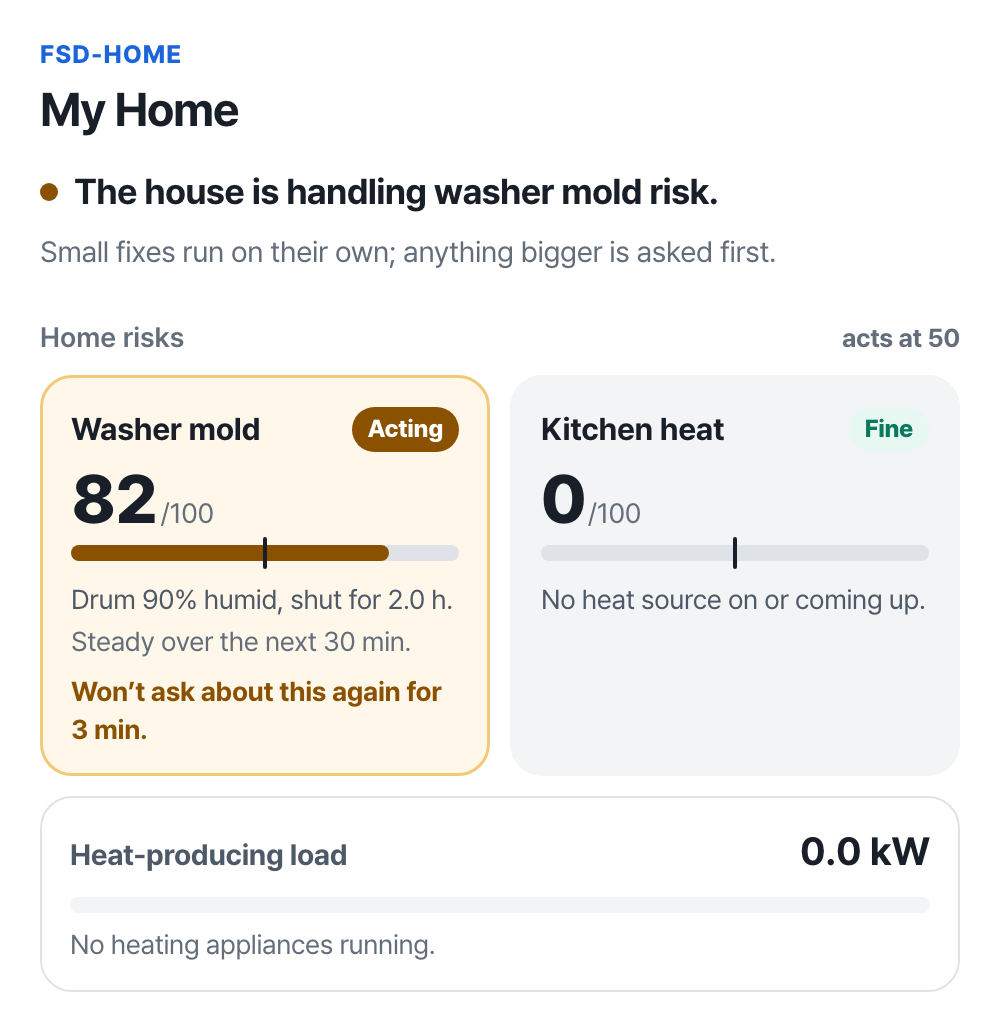
\includegraphics[width=0.72\columnwidth]{figures/uc1-mold.png}
\caption{Use Case 1: the mold index at 82 triggers Level~1 actions without asking.}
\label{fig:uc1}
\end{figure}

\subsection{Use Case 2: Per-Action Approval for Kitchen Overload}
\textbf{Satisfies:} FR-2, FR-3 (Level~2), FR-4.
\begin{enumerate}
    \item Choose \emph{Demo controls} $\rightarrow$ \emph{Dryer + dinner soon}. The dryer is running, the kitchen is at 31.5~$^\circ$C, the refrigerator compressor runs at 80\%, and a cooking session starts in 20 minutes.
    \item The Thermal Overload Index reaches 100. The engine turns on the range hood and pre-cools the kitchen (Level~1) without asking.
    \item Two Level~2 actions remain. The screen shows \emph{two separate cards}, ``Balcony Dryer $\cdot$ Stop the dryer'' and ``Kitchen Cooktop $\cdot$ Preheat the cooktop'', each with its own request identifier, Yes/No buttons and a five-minute countdown (Fig.~\ref{fig:uc2}). The first question is also read aloud.
\end{enumerate}

\begin{figure}[htbp]
\centering
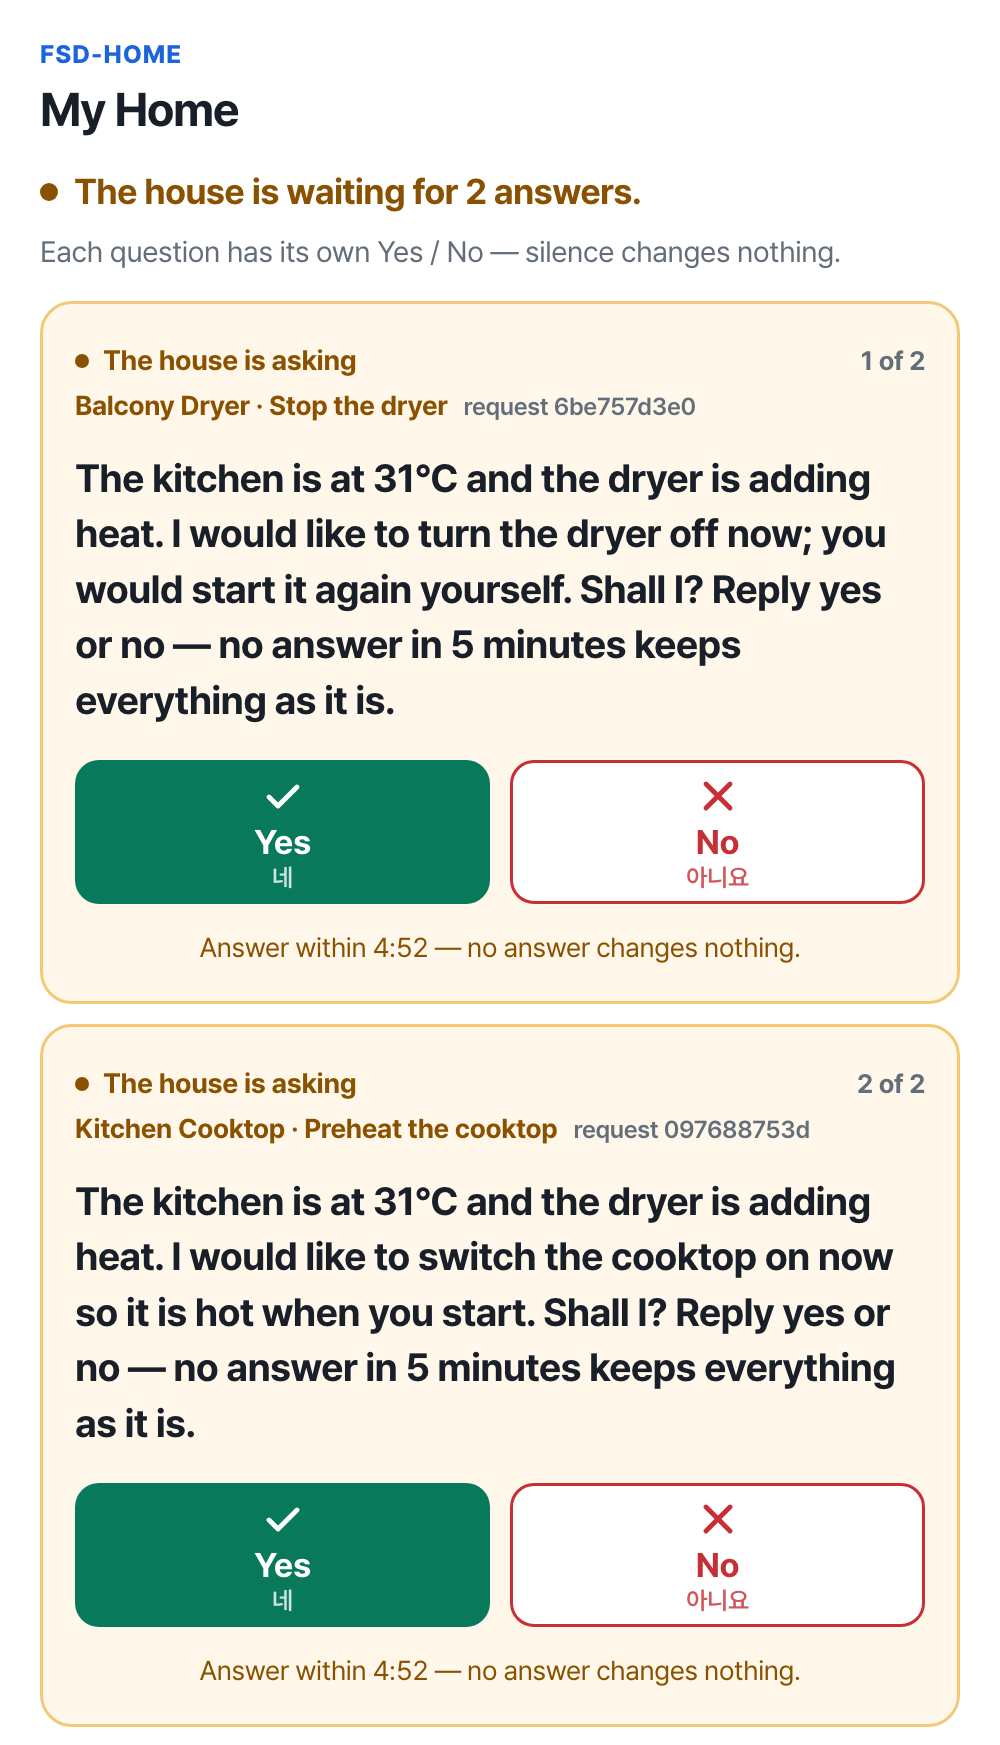
\includegraphics[width=0.72\columnwidth]{figures/uc2-approvals.png}
\caption{Use Case 2: one approval card per Level~2 action, each with its own countdown.}
\label{fig:uc2}
\end{figure}

\subsection{Use Case 3: Confirming, Revalidation and the Cooktop Interlock}
\textbf{Satisfies:} FR-4, FR-5, FR-6.
\begin{enumerate}
    \item In the state of Use Case~2, press \emph{Yes} on the dryer card. The engine revalidates the request (still valid, overload still active, dryer still on), records the intent, stops the dryer and records the outcome. The message reads ``You said yes, so I turned the dryer off''.
    \item Removing the dryer's 1.8~kW clears the overload; the house sends one reminder that the dryer can be restarted by hand. It never restarts the dryer itself.
    \item Press \emph{Yes} on the cooktop card. Because the overload has cleared, the cooktop is revalidated against the meal instead: someone is at home, cooking is still scheduled, and the cooktop is still off. The cooktop switches on.
    \item A red banner shows that the cooktop is being watched: it is waiting for cooking to start, will switch off if no cooking begins within 5 minutes of the scheduled start, and will switch off after 30 minutes at most (Fig.~\ref{fig:uc3}). The cooktop's own load raises the thermal index again, which the risk card reports truthfully.
\end{enumerate}

\begin{figure}[htbp]
\centering
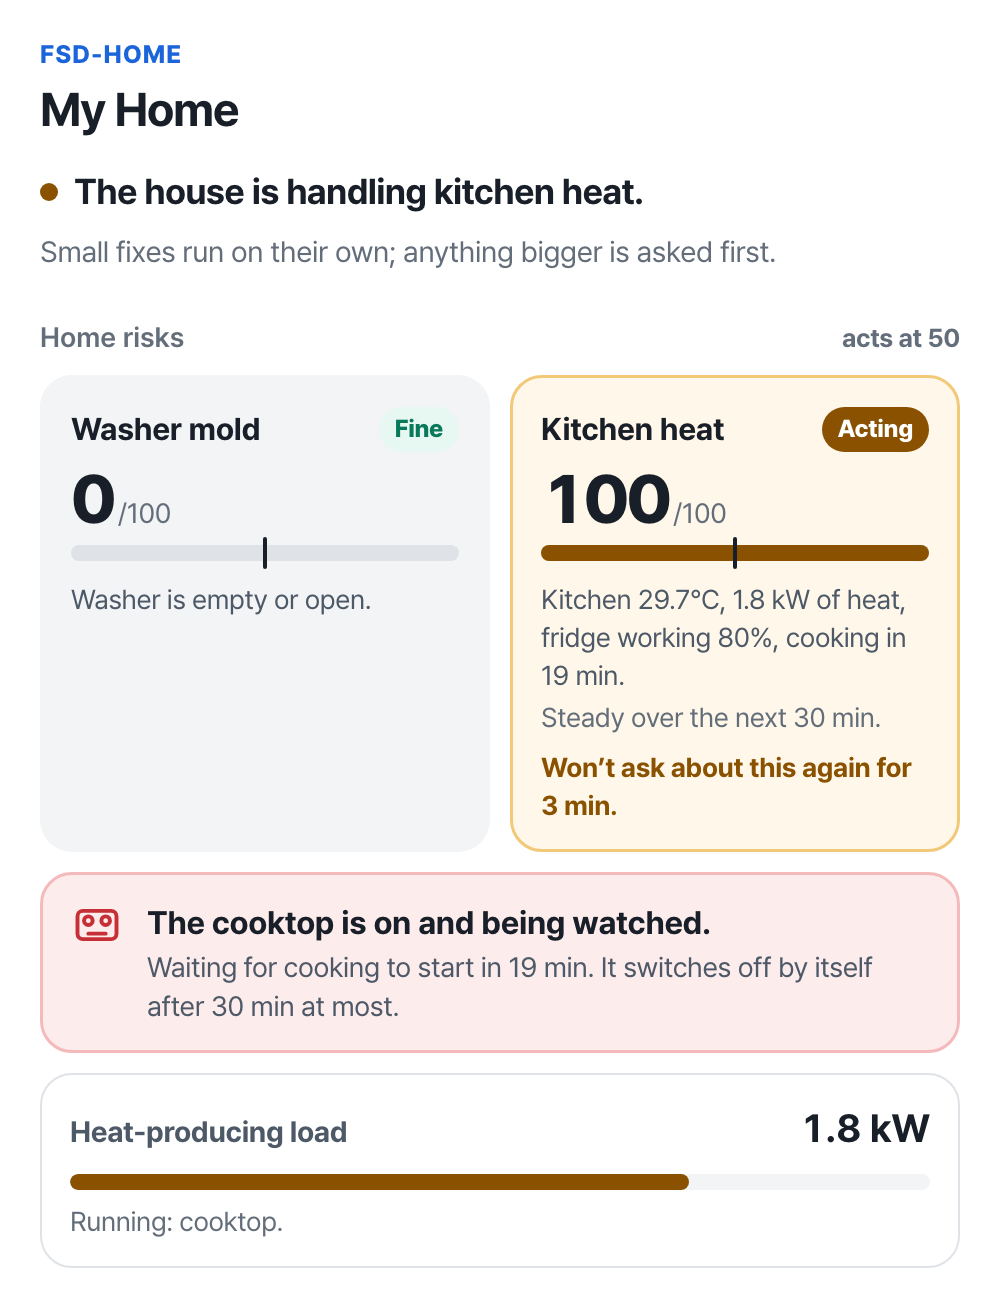
\includegraphics[width=0.72\columnwidth]{figures/uc3-guard.png}
\caption{Use Case 3: after both confirmations the cooktop is on and watched by the interlock.}
\label{fig:uc3}
\end{figure}

\subsection{Use Case 4: Declining or Not Answering}
\textbf{Satisfies:} FR-4, FR-5 (fail-safe default).
\begin{enumerate}
    \item Load \emph{Dryer + dinner soon} again and press \emph{No} on both cards --- or leave them unanswered for five minutes.
    \item Neither the dryer nor the cooktop changes. The Level~1 actions that already ran stay in effect, and the message names only the appliances that were left alone.
    \item The kitchen card now reads ``Won't ask about this again for 30 min'': the quiet period is visible, and the live score stays on screen during it (Fig.~\ref{fig:uc4}).
    \item An answer that arrives after the deadline is treated exactly like no answer.
\end{enumerate}

\begin{figure}[htbp]
\centering
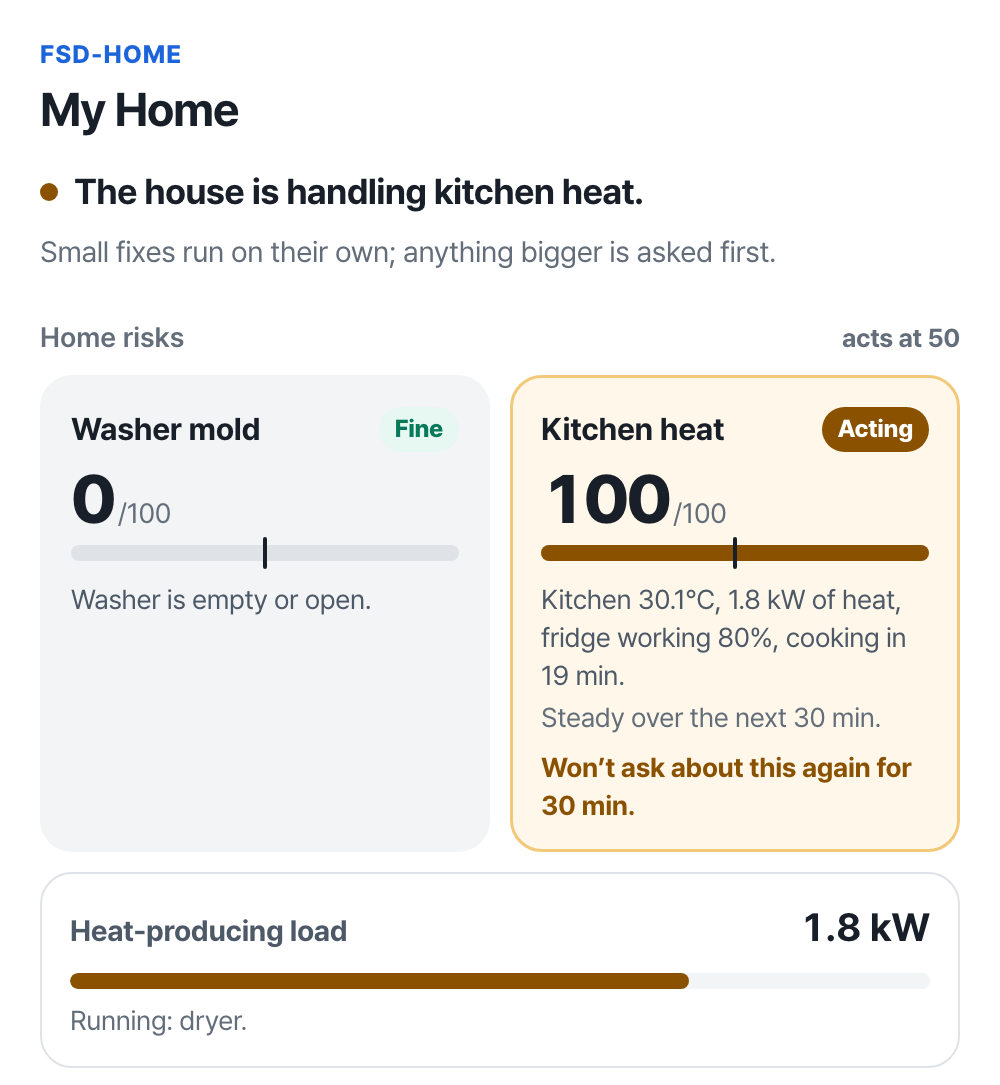
\includegraphics[width=0.72\columnwidth]{figures/uc4-quiet.png}
\caption{Use Case 4: after a decline nothing changes and the 30-minute quiet period is shown.}
\label{fig:uc4}
\end{figure}

\subsection{Use Case 5: A Stale ``Yes'' Is Refused}
\textbf{Satisfies:} FR-5 (pre-execution revalidation).
\begin{enumerate}
    \item A cooktop request is pending (Use Case~2).
    \item Before the user answers, the situation changes: the resident leaves home, the cooking session is removed from the calendar, or someone switches the cooktop on by hand.
    \item The user presses \emph{Yes}. Revalidation fails, the adapter is not called, an \texttt{action.blocked} row records the reason, and the user is told why, e.g.\ ``nobody is home to watch the cooktop''.
\end{enumerate}
These paths are exercised by the unit tests in \texttt{tests/test\_fr456.py} (for example \texttt{test\_preheat\_cooktop\_is\_refused\_when\_nobody\_is\_home} and \texttt{test\_a\_yes\_after\_the\_risk\_clears\_is\_refused\_with\_a\_reason}).

\subsection{Use Case 6: Tracing a Decision in the Safety Log}
\textbf{Satisfies:} FR-6.
\begin{enumerate}
    \item After Use Case~3, scroll to the \emph{Safety log} on the home screen, or call \texttt{GET /api/audit}.
    \item Each row shows the time, a plain-language event and the underlying \texttt{event\_type}. Rows that belong to one request share its identifier, so the chain \emph{You said yes} $\rightarrow$ \emph{About to act} $\rightarrow$ \emph{Done} can be followed for each action (Fig.~\ref{fig:uc6}).
    \item The log cannot be edited: an \texttt{UPDATE} or \texttt{DELETE} on \texttt{audit\_log} is aborted by the database triggers.
\end{enumerate}

\begin{figure}[htbp]
\centering
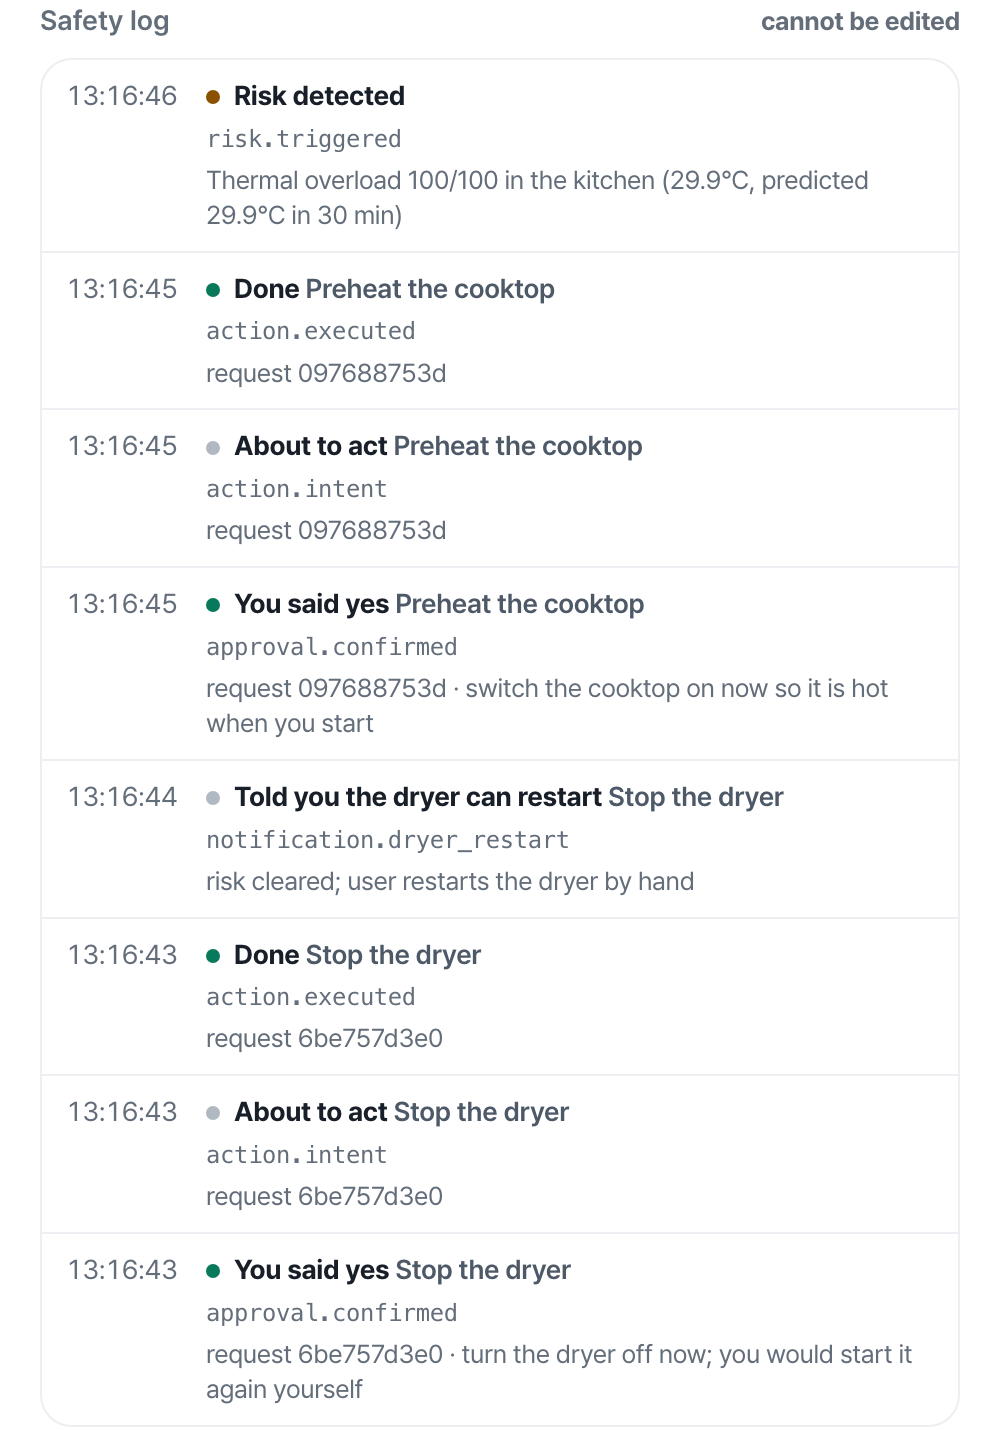
\includegraphics[width=0.72\columnwidth]{figures/uc6-audit.png}
\caption{Use Case 6: the Safety log links each approval to the intent and the device outcome.}
\label{fig:uc6}
\end{figure}

\subsection{Use Case 7: Running Without the Language Model}
\textbf{Satisfies:} NFR-1, NFR-2.
\begin{enumerate}
    \item Start the system with the model pointed at an unreachable address: \texttt{LLM\_BASE\_URL=http://127.0.0.1:9 python run.py --scenario oven}.
    \item The engine logs \texttt{proactive.decide\_fallback} and the rules choose the Level~1 actions. Approval cards, revalidation, the interlock and the audit trail behave exactly as in Use Cases~2--4.
    \item \texttt{python -m unittest discover -s tests} (276 tests) and \texttt{python -m eval.run} verify the same behaviour without any network access.
\end{enumerate}

\begin{thebibliography}{00}
\bibitem{lgwhitepaper2024} LG Electronics, ``Affectionate Intelligence and Zero Labor Home Vision,'' LG ThinQ Ecosystem Whitepaper, 2024.
\bibitem{samsung2026a} Samsung Electronics, ``Home Companion: Comprehension of Samsung Bespoke AI 2026,'' Jan. 2026.
\bibitem{epa2022} U.S. Environmental Protection Agency (EPA), ``A Brief Guide to Mold, Moisture and Your Home,'' EPA 402-K-02-003, 2022.
\bibitem{ashrae2023} ASHRAE, ``Standard 55: Thermal Environmental Conditions for Human Occupancy,'' ASHRAE, 2023.
\bibitem{yuan2024} T. Yuan et al., ``R-Judge: Benchmarking Safety Risk Awareness for LLM Agents,'' arXiv:2401.10019, 2024.
\bibitem{pradhan2020} A. Pradhan, A. Lazar, and L. Findlater, ``Use of Intelligent Voice Assistants by Older Adults,'' ACM TOCHI, vol. 27, no. 4, 2020.
\bibitem{msit2026} Ministry of Science and ICT, ``2025 Survey on the Digital Divide,'' KDI Economic Info Center, Mar. 2026.
\bibitem{moneytoday2026} Money Today, ``2025 Digital Divide Survey: Competency Level Analysis,'' Mar. 2026.
\bibitem{maeil2026} Maeil Business Newspaper, ``Home Appliance Usability Survey for Consumers 50+,'' 2026.
\bibitem{seoulfire2020} Seoul Metropolitan Fire Headquarters, ``2019 Residential Fire Statistics Analysis,'' 2020.
\bibitem{nfa2025} National Fire Agency, ``Chuseok Holiday Fire Safety Bulletin,'' Seoul Shinmun, 2025.
\bibitem{who2009} World Health Organization (WHO), ``WHO Guidelines for Indoor Air Quality: Dampness and Mould,'' 2009.
\bibitem{lgspec2026} LG Electronics, ``LG ThinQ Platform Specifications,'' Official Whitepaper, 2026.
\bibitem{samsung2026b} Samsung India, ``2026 Range of Bespoke AI Appliances,'' Press Release, 2026.
\bibitem{wcag2023} W3C, ``Web Content Accessibility Guidelines (WCAG) 2.2,'' W3C Recommendation, 2023.
\end{thebibliography}

\end{document}
